\documentclass[a4paper,11pt]{article}
\usepackage[utf8]{inputenc}
\usepackage[backend=biber]{biblatex}
\addbibresource{referencias.bib}
\usepackage[a4paper, top=3cm, bottom=3cm, left=3cm, right=3cm]{geometry}
\usepackage[T1]{fontenc}
\usepackage{multirow}
\usepackage{booktabs}
\usepackage{graphicx}
\usepackage{rotating}
\usepackage{float}
\usepackage{fancyhdr}
\usepackage{setspace}
\usepackage{listings}
\usepackage{ragged2e} % for \justifying
\usepackage{enumitem} % better lists
\usepackage{hyperref} % hyperlinks
\usepackage{xcolor}
\usepackage{amsmath,amssymb,textcomp}
\usepackage{multicol}
\usepackage{tikz}
\usepackage{pdflscape} % en el preámbulo

% Header & footer
\pagestyle{fancy}
\fancyhf{}
\lhead{\footnotesize EQUIPO 1 }
\rhead{\footnotesize 5CV3} 
\cfoot{\footnotesize \thepage}
\setlength{\parindent}{0in}

\begin{document}
\vspace{0.4cm}

\begin{titlepage}
    \centering
    {\bfseries\LARGE Escuela Superior de Cómputo \par}
    \vspace{1cm}
    {\scshape\Large REDES DE COMPUTADORAS \par}
    \vspace{5cm}
    {\scshape\Huge \textbf{Práctica de laboratorio:} \par}
    {\scshape\Huge Configuración básica de routers \par}
    \vfill
    {\Large \textbf{Por el equipo 1:} \par}
    {\Large Barrera Puente Eric Alejandro \par}
    {\Large Diaz Villegas Ramón Alexis \par}
    {\Large Sánchez Gómez Alan Iván \par}
    \vspace{1cm}
    {\Large \textbf{Grupo: 5CV3} \par}
    \vfill
    {\Large 24 de Septiembre, 2025 \par}
\end{titlepage}

\tableofcontents %índice
\newpage

\listoffigures
\newpage

\justify
\section{Desarrollo de la práctica}
\subsection{Configuración de nombres de routers}
Para el desarrollo de la práctica, se decidió manejar los nombres definidos por
defecto en la práctica
\begin{itemize}
    \item R1-ISP (Router 1 - Internet Service Provider)
    \item R2-Central (Router 2 - Central)
    \item S1-Central (Switch 1 - Central)
\end{itemize}

\begin{figure}[h]
    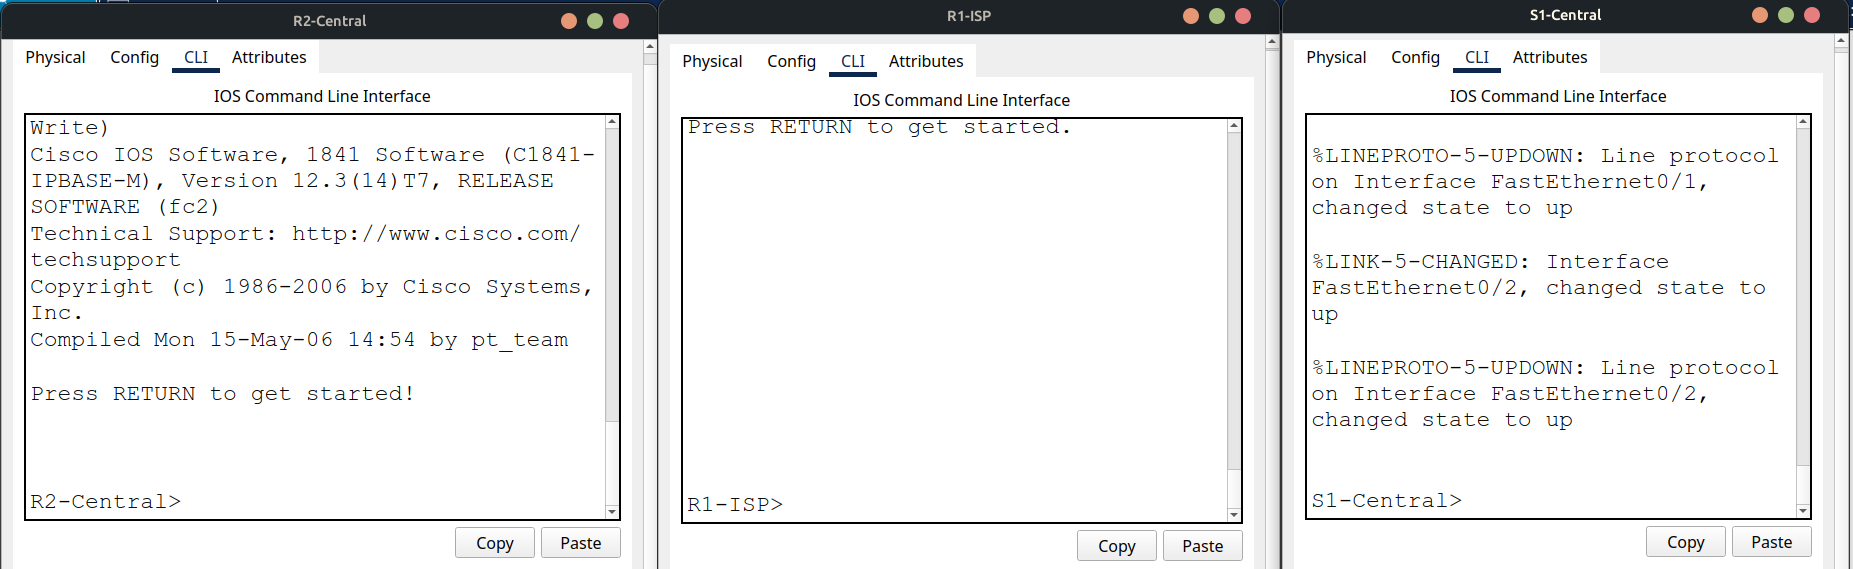
\includegraphics[width=1\textwidth]{images/figure1.png}
    \caption{Configuración de los nombres de Routers}
\end{figure}

\subsection{Configuración de interfaces}
Para garantizar una transmisión de datos exitosa, es necesario asignar
direcciones IP a las interfaces \texttt{FastEthernet0/0} y \texttt{Serial0/0/0}
de los routers R1-ISP y R2-Central. Para ello retomamos las configuraciones
indicadas en la práctica \textit{“1\_2 IOS configuration modes”}.
\vspace{0.2cm}

Así, comenzamos configurando \texttt{R1-ISP}:

\begin{itemize}
    \item Entramos al modo \textit{EXEC privilegiado}.
    \item Usamos el comando \texttt{configure terminal} para acceder al modo de
          configuración global.
    \item Ingresamos a la interfaz que se va a configurar.
    \item Asignamos la dirección IP y la máscara de subred.
    \item Ejecutamos el comando \texttt{no shutdown}.
    \item Salimos y aplicamos los cambios con \texttt{write memory}.
\end{itemize}

\begin{figure}[h]
    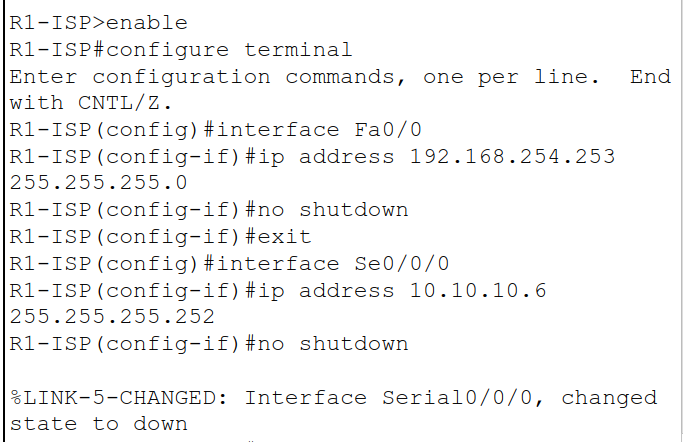
\includegraphics[width=1\textwidth]{images/ip_r1.png}
    \caption{Configuración de la interfaz Fa0/0 y Se0/0/0 de R1-ISP}
\end{figure}

\newpage
Así, obtenemos el siguiente resultado para el \texttt{R1-ISP}:

\begin{figure}[h]
    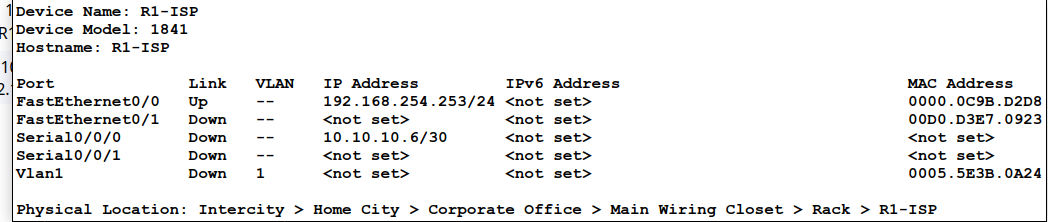
\includegraphics[width=1\textwidth]{images/ip_r1_result.png}
    \caption{Resultado de configuración de la interfaz Fa0/0 y Se0/0/0 de R1-ISP}
\end{figure}

Repetimos el mismo proceso para R2-Central siguiendo el diagrama y las Ip
propuestas

\newpage
\begin{figure}[h]
    \centering
    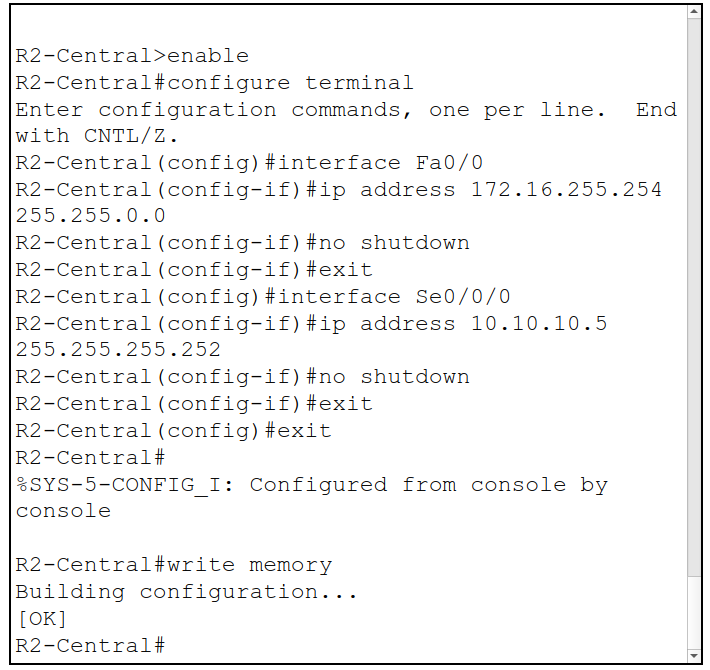
\includegraphics[width=0.85\textwidth]{images/ip_r2.png}
    \caption{Configuración de la interfaz Fa0/0 y Se0/0/0 de R2-Central}
\end{figure}

Obteniendo de esta manera, el siguiente resultado para el \texttt{R2-Central}:

\begin{figure}[h]

    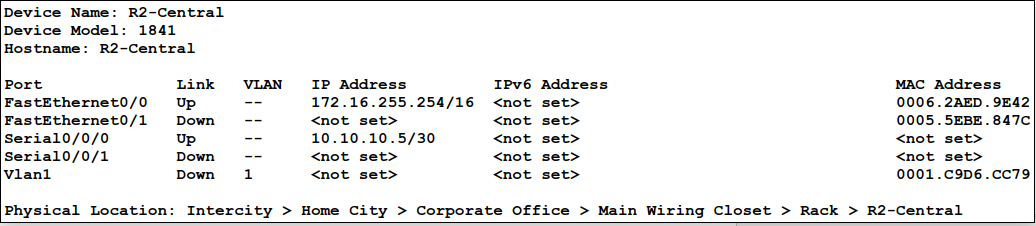
\includegraphics[width=1\textwidth]{images/ip_r2_result.png}
    \caption{Resultado de configuración de la interfaz Fa0/0 y Se0/0/0 de R2-Central}
\end{figure}

Al terminar tendremos una conexión estable y funcional capaz de enviar y
recibir mensajes. A continuación, en la figura 6, se observa la topología con
las configuraciones de Ip como labels.

\begin{figure}[h]
    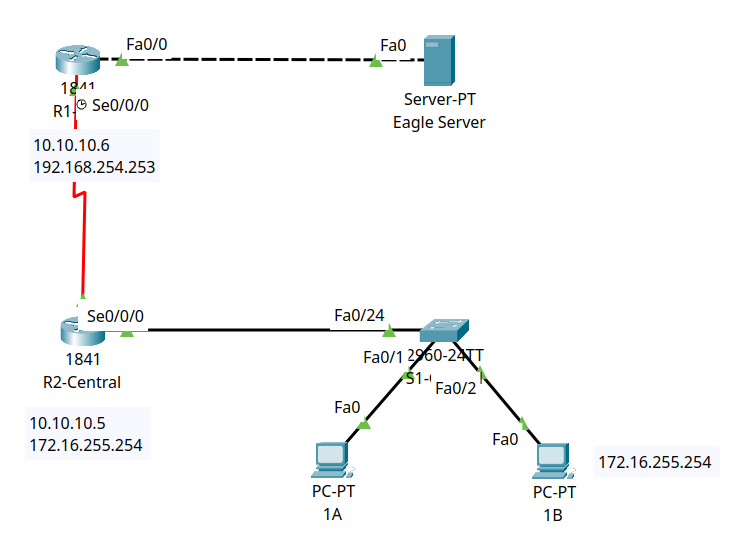
\includegraphics[width=1 \textwidth]{images/config_diagram.png}
    \caption{Esquema de conexiones de la red e IP's propuestas}
\end{figure}

\newpage

\subsection{Configuración de contraseñas y banners}

En esta práctica se configuraron las contraseñas y banners en los routers y
switches para garantizar la seguridad de acceso.

\begin{itemize}
    \item \textbf{Configuración de un router:}
          \begin{enumerate}
              \item Acceder al router (R1-ISP) y entrar al modo privilegiado con \texttt{enable}.
              \item Ingresar al modo de configuración global: \texttt{configure terminal}.
              \item Configurar la contraseña encriptada para el modo privilegiado: \texttt{enable
                        secret class}.
              \item Configurar la línea de consola:
                    \begin{itemize}
                        \item Entrar al modo de línea: \texttt{line con 0}.
                        \item Asignar la contraseña: \texttt{password cisco}.
                        \item Activar la solicitud de contraseña: \texttt{login}.
                        \item Salir al modo global: \texttt{exit}.
                    \end{itemize}
              \item Configurar las líneas VTY (acceso remoto):
                    \begin{itemize}
                        \item Entrar al modo de línea: \texttt{line vty 0 4}.
                        \item Asignar la contraseña: \texttt{password cisco}.
                        \item Activar la solicitud de contraseña: \texttt{login}.
                        \item Salir al modo global: \texttt{exit}.
                    \end{itemize}
              \item Configurar un banner de mensaje: \texttt{banner motd \#This is a secure
                        system.\#}.
              \item Guardar la configuración en la memoria NVRAM: \texttt{copy running-config
                        startup-config}.
          \end{enumerate}
          \vspace{0.5cm}

          \begin{figure}[h]
              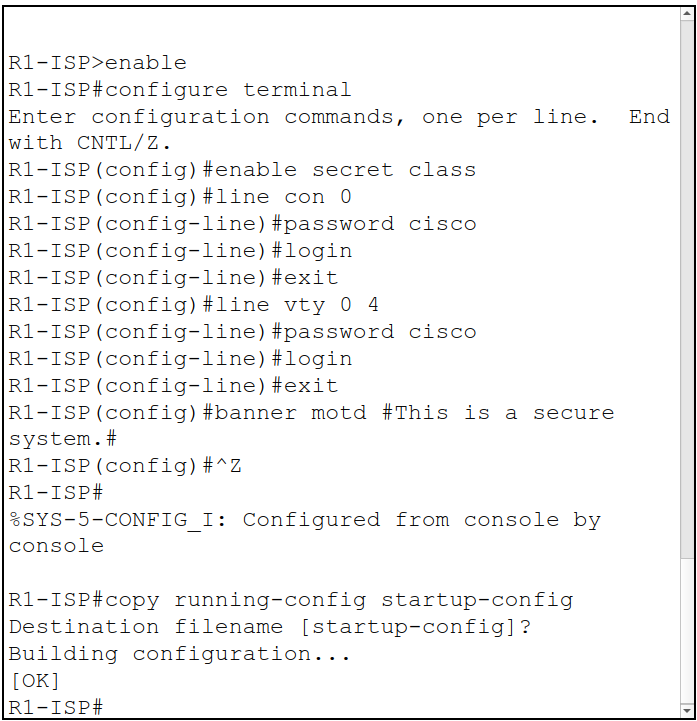
\includegraphics[width=1\textwidth]{images/password_banner.png}
              \caption{Establecimiento de contraseña y banner para R1-ISP}
          \end{figure}

    \item \textbf{Verificación:}
          \begin{itemize}
              \item Verificar la configuración con \texttt{show running-config}.
              \item Probar el acceso con las contraseñas configuradas y observar el banner.
          \end{itemize}

          \begin{figure}[h]
              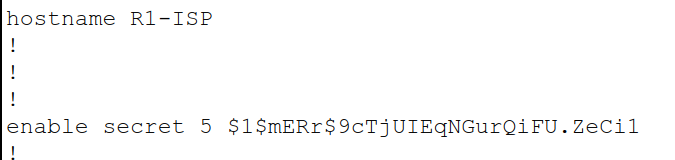
\includegraphics[width=1\textwidth]{images/secret_result.png}
              \caption{Visualización de la contraseña establecida con \emph{enable secret class}}
          \end{figure}

          \begin{figure}[h]
              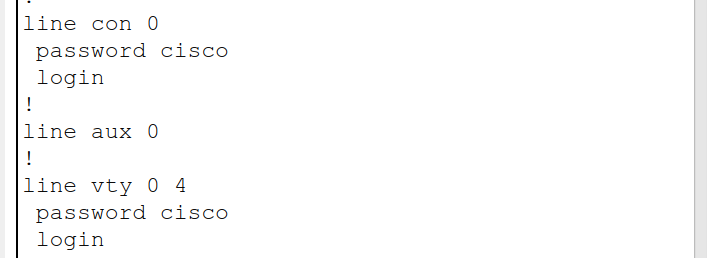
\includegraphics[width=1\textwidth]{images/nosecret_result.png}
              \caption{Visualización de la contraseña establecida con \emph{password cisco}}
          \end{figure}

          \newpage
    \item \textbf{Configuración en otros dispositivos:}
          \begin{itemize}
              \item Repetir los pasos anteriores para el segundo router y el switch.
          \end{itemize}

          Al terminar, obtendremos una pantalla que nos mostrará el banner y pedirá
          contraseña para usar el command prompt en modo usuario y también para entrar a
          modo exec privilegiado

          \begin{figure}[h]
              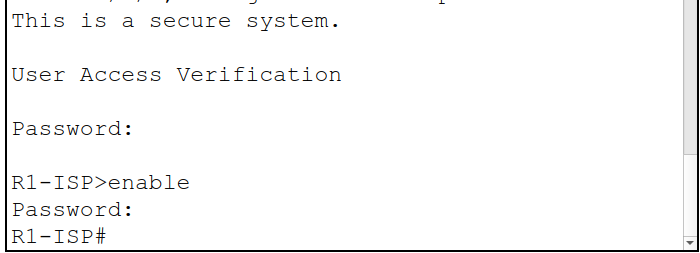
\includegraphics[width=1\textwidth]{images/initial_prompt.png}
              \caption{Visualización de banner y de solicitud de password al configurar router}
          \end{figure}

\end{itemize}

\subsection{Prueba de conectividad con \texttt{ping}}

Una vez configuradas las direcciones IP en los dispositivos de la red y
asegurada la correcta asignación de contraseñas y banners, se procedió a
verificar la conectividad entre los equipos utilizando el comando \texttt{ping}
desde la computadora.

La prueba consistió en abrir la ventana de comandos de la PC y ejecutar el
siguiente comando:

\begin{center}
    \texttt{ping <dirección\_IP\_del\_router>}
\end{center}

Si la configuración de red es correcta y no existen fallos en las conexiones
físicas o lógicas, el resultado esperado son respuestas exitosas del destino,
lo que indica que la comunicación entre la computadora y el router funciona
adecuadamente. En caso contrario, se revisarían los parámetros de configuración
de interfaces, direcciones IP o el estado de las conexiones.

\subsubsection*{Pasos realizados}
\begin{enumerate}
    \item Acceder a la computadora en Packet Tracer.
    \item Abrir la pestaña \texttt{Desktop} y seleccionar \texttt{Command Prompt}.
    \item Ejecutar el comando \texttt{ping} seguido de la dirección IP del router o
          dispositivo de destino.
    \item Observar si la respuesta es satisfactoria (respuesta exitosa) o si existen
          pérdidas de paquetes.
\end{enumerate}

Además del comando \texttt{ping}, Packet Tracer permite verificar la
conectividad de forma gráfica arrastrando un mensaje (en modo simulación) desde
la computadora hacia el dispositivo de destino, observando así si el paquete
llega correctamente. \vspace{1cm}

\begin{figure}[h]
    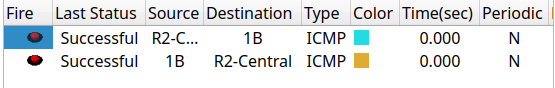
\includegraphics[width=1\textwidth]{images/connectivity_test.png}
    \caption{Prueba de conexión con el icono de mensaje de Packet Tracer}
\end{figure}

\begin{figure}[H]
    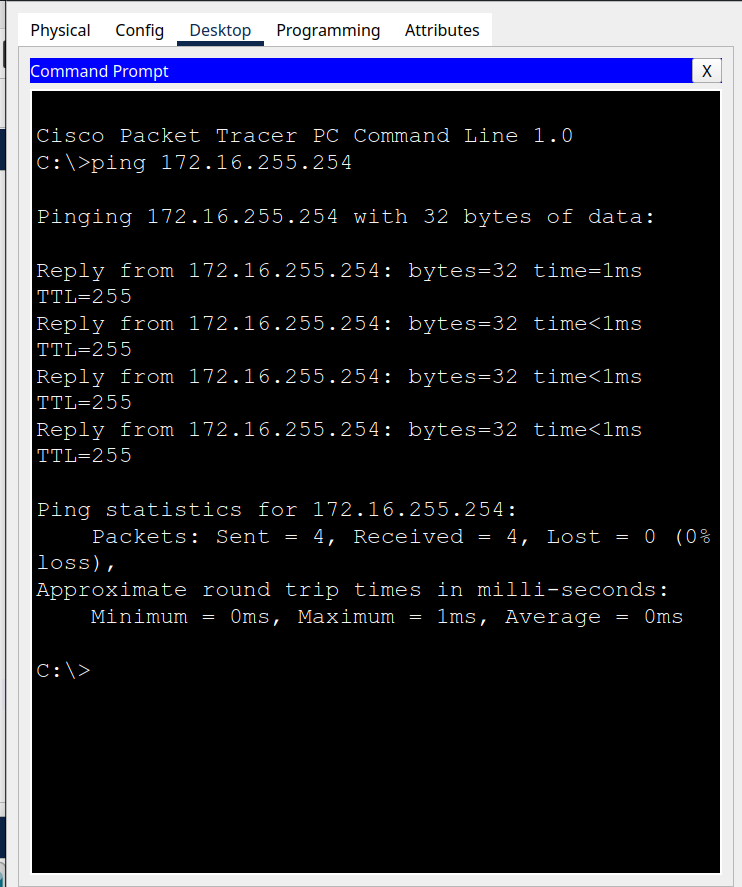
\includegraphics[width=1\textwidth]{images/ping.png}
    \caption{Prueba de conexión con el comando \emph{ping}}
\end{figure}

\subsection{Conclusión de la práctica al 100\%}
En esta sección únicamente se hace anexo de la captura con el 100\% completado
de la práctica por medio del evaluador de packet tracer

\begin{figure}[H]
    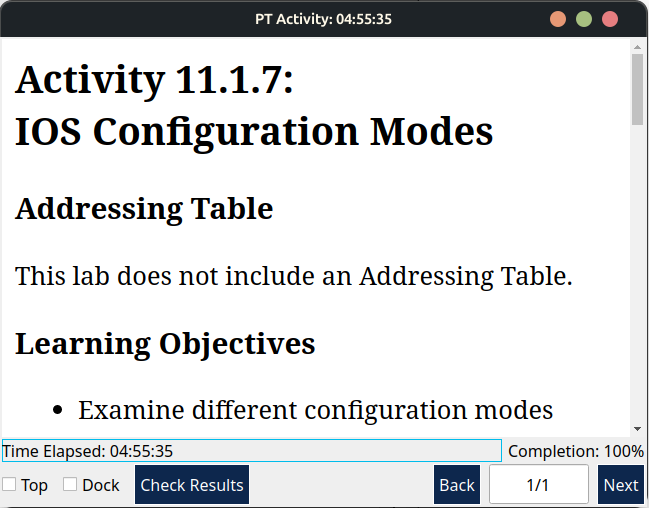
\includegraphics[width=1\textwidth]{images/completion.png}
\end{figure}

\section{Conclusiones}
\begin{itemize}
    \item \textbf{Barrera Puente Eric Alejandro:}
          Durante esta práctica de laboratorio logramos aplicar de manera efectiva los conceptos teóricos de redes de computadoras para construir y configurar una red funcional. Al trabajar con Packet Tracer, pudimos simular un entorno real y poner en práctica habilidades esenciales como:
          \begin{itemize}
              \item \textbf{Asignación de direcciones IP:} Comprendimos cómo realizar la configuración correcta de las interfaces.
              \item \textbf{Conectividad y diagnóstico:} Utilizamos herramientas como el comando \texttt{ping} y la simulación de Packet Tracer para verificar la conectividad y solucionar posibles errores de configuración.
              \item \textbf{Seguridad básica:} Aprendimos que la configuración de contraseñas para los diferentes modos de usuario (consola, VTY y modo privilegiado), así como el uso de banners, son una primera e indispensable capa de seguridad para proteger los dispositivos de red contra accesos no autorizados.
          \end{itemize}

    \item \textbf{Díaz Villegas Ramón Alexis:}
          Durante el desarrollo de esta práctica experimenté diversas dificultades que me permitieron comprender mejor el funcionamiento de los dispositivos de red. Inicialmente tuve problemas para acceder al modo de configuración terminal, ya que no comprendía la diferencia entre el modo usuario (\texttt{Router>}) y el modo privilegiado (\texttt{Router\#}). Esta confusión me llevó a intentar ejecutar comandos de configuración sin los privilegios necesarios, generando errores de sintaxis.

          Otra complicación fue el manejo de las contraseñas. Al principio no entendía
          por qué no se mostraban los caracteres al escribirlas, lo cual es un
          comportamiento normal de seguridad en los sistemas de red. También tuve
          dificultades para distinguir entre los diferentes tipos de contraseñas:
          \texttt{enable secret} (encriptada) y las contraseñas de línea (inicialmente en
          texto plano). La configuración del servicio de encriptación de contraseñas
          (\texttt{service password-encryption}) fue reveladora, ya que pude observar
          directamente cómo las contraseñas cambiaron de texto plano a formato
          encriptado.

          Esta experiencia práctica me ayudó a entender la importancia de la seguridad en
          las configuraciones de red. Finalmente, comprendí que la configuración de
          dispositivos requiere precisión, paciencia y un entendimiento claro de los
          diferentes modos de operación.

    \item \textbf{Sánchez Gómez Alan Iván:}
          Durante esta práctica se generó una red local con dispositivos finales interconectados a un router. Si realizamos una pequeña abstracción, este escenario puede representar la configuración de red de una oficina o de una casa.

          Es fundamental proteger los cambios que se pueden realizar en los dispositivos
          y controlar quiénes tienen acceso a dichas configuraciones, ya que una
          configuración inicial sin medidas de defensa queda expuesta a riesgos.

          Al concluir esta práctica, pudimos establecer los pasos necesarios para
          configurar un router y los dispositivos finales de manera que reciban la
          conexión, permitiendo una comunicación fluida. Asimismo, comprendimos la
          importancia de agregar una capa adicional de seguridad a la configuración para
          garantizar un entorno más confiable.
\end{itemize}

\end{document}
